\documentclass{article}\usepackage[]{graphicx}\usepackage[]{color}
%% maxwidth is the original width if it is less than linewidth
%% otherwise use linewidth (to make sure the graphics do not exceed the margin)
\makeatletter
\def\maxwidth{ %
  \ifdim\Gin@nat@width>\linewidth
    \linewidth
  \else
    \Gin@nat@width
  \fi
}
\makeatother

\definecolor{fgcolor}{rgb}{0.345, 0.345, 0.345}
\newcommand{\hlnum}[1]{\textcolor[rgb]{0.686,0.059,0.569}{#1}}%
\newcommand{\hlstr}[1]{\textcolor[rgb]{0.192,0.494,0.8}{#1}}%
\newcommand{\hlcom}[1]{\textcolor[rgb]{0.678,0.584,0.686}{\textit{#1}}}%
\newcommand{\hlopt}[1]{\textcolor[rgb]{0,0,0}{#1}}%
\newcommand{\hlstd}[1]{\textcolor[rgb]{0.345,0.345,0.345}{#1}}%
\newcommand{\hlkwa}[1]{\textcolor[rgb]{0.161,0.373,0.58}{\textbf{#1}}}%
\newcommand{\hlkwb}[1]{\textcolor[rgb]{0.69,0.353,0.396}{#1}}%
\newcommand{\hlkwc}[1]{\textcolor[rgb]{0.333,0.667,0.333}{#1}}%
\newcommand{\hlkwd}[1]{\textcolor[rgb]{0.737,0.353,0.396}{\textbf{#1}}}%
\let\hlipl\hlkwb

\usepackage{framed}
\makeatletter
\newenvironment{kframe}{%
 \def\at@end@of@kframe{}%
 \ifinner\ifhmode%
  \def\at@end@of@kframe{\end{minipage}}%
  \begin{minipage}{\columnwidth}%
 \fi\fi%
 \def\FrameCommand##1{\hskip\@totalleftmargin \hskip-\fboxsep
 \colorbox{shadecolor}{##1}\hskip-\fboxsep
     % There is no \\@totalrightmargin, so:
     \hskip-\linewidth \hskip-\@totalleftmargin \hskip\columnwidth}%
 \MakeFramed {\advance\hsize-\width
   \@totalleftmargin\z@ \linewidth\hsize
   \@setminipage}}%
 {\par\unskip\endMakeFramed%
 \at@end@of@kframe}
\makeatother

\definecolor{shadecolor}{rgb}{.97, .97, .97}
\definecolor{messagecolor}{rgb}{0, 0, 0}
\definecolor{warningcolor}{rgb}{1, 0, 1}
\definecolor{errorcolor}{rgb}{1, 0, 0}
\newenvironment{knitrout}{}{} % an empty environment to be redefined in TeX

\usepackage{alltt}
\usepackage[unicode=true]{hyperref}
\usepackage{geometry}
\geometry{tmargin=1in,bmargin=1in,lmargin=1in,rmargin=1in}
\IfFileExists{upquote.sty}{\usepackage{upquote}}{}
\begin{document}
\title{PS 2}
\author{Chris Gagne}
\date{September 20th 2017}

\maketitle



\section*{4.1: CartPole Experiments}

\subsection*{Methods}

I ran the following experiments (with the default learning rate of 0.001): 

\begin{knitrout}
\definecolor{shadecolor}{rgb}{0.969, 0.969, 0.969}\color{fgcolor}\begin{kframe}
\begin{alltt}
python train_pg.py CartPole-v0 -n 100 -b 1000 -e 5 -dna \textbackslash{}
--exp_name sb_no_rtg_dna -l 1 -s 32 --seed 101

python train_pg.py CartPole-v0 -n 100 -b 1000 -e 5 -rtg -dna \textbackslash{} 
--exp_name sb_rtg_dna -l 1 -s 32 --seed 101

python train_pg.py CartPole-v0 -n 100 -b 1000 -e 5 -rtg \textbackslash{}
--exp_name sb_rtg_na -l 1 -s 32 --seed 101

python plot.py \textbackslash{}
data/sb_no_rtg_dna_CartPole-v0_20-09-2017_10-14-40 \textbackslash{}
data/sb_rtg_dna_CartPole-v0_20-09-2017_10-18-19 \textbackslash{}
data/sb_rtg_na_CartPole-v0_20-09-2017_10-26-17

python train_pg.py CartPole-v0 -n 100 -b 5000 -e 5 -dna \textbackslash{} 
--exp_name lb_no_rtg_dna -l 1 -s 32 --seed 101

python train_pg.py CartPole-v0 -n 100 -b 5000 -e 5 -rtg -dna \textbackslash{} 
--exp_name lb_rtg_dna -l 1 -s 32 --seed 101

python plot.py \textbackslash{}
data/lb_no_rtg_dna_CartPole-v0_20-09-2017_10-36-39 \textbackslash{} 
data/lb_rtg_dna_CartPole-v0_20-09-2017_10-49-43

\end{alltt}
\end{kframe}
\end{knitrout}

\noindent Before running these experiments, I generated a bunch of observations from each environment by randomly choosing actions. I calculated the mean and std for observations. I saved this out and used it to normalize observations for each environment. I do this after observing each action in the gym. I also experimented with different network sizes, but realized that 1 hidden layer and 32 units was sufficient. 

\subsection*{Results}

\begin{itemize}
 \item The reward to go estimator seemed to have helped at least for this random seed. Using it achieved asymptotic performance quicker, and may have reduced the variance of the gradient a bit, judging by the variance in the average return. In theory, I can't imagine a reason why not having the reward to go would be better. (This was pointed out in lecture). See Figure 1. 
 \item Advantage centering did not seem to help in this case. Intuitively, advantage centering rescales the returns so that they are relative to one an another. These act as weights applied to the log likelihood to emphasize (state,action) pairs that were particularly good in the long run. This should help in cases where there is a wide range of possible returns. Since CartPole is such a short game however perhaps the relative importance of returns with and without advantage centering is similar enough. See Figure 1.
 \item Batch size seems reduces the variance of the policy gradient, as judged by variance in average return. It also seems to have sped up the rate at which the algorithm achieves assymptomic performance, which is not surprising since it uses more data at each step. See Figure 2. 
 \end{itemize}


\begin{figure}
  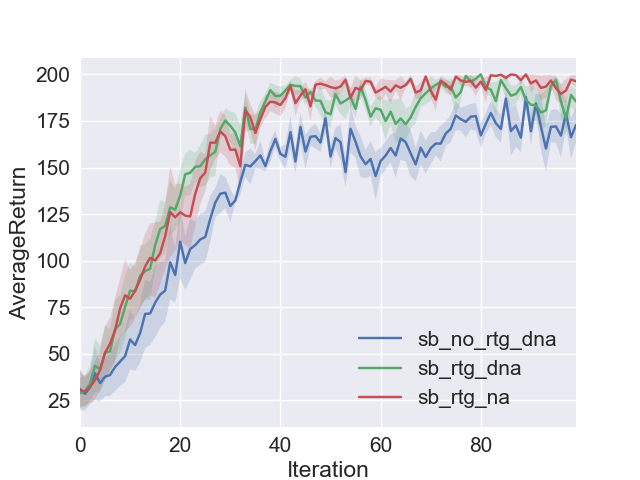
\includegraphics[width=\linewidth]{figures/sb_experiments_4.png}
  \caption{CartPole (batch size 1000)}
  \label{sb comparisons}
\end{figure}

\begin{figure}
  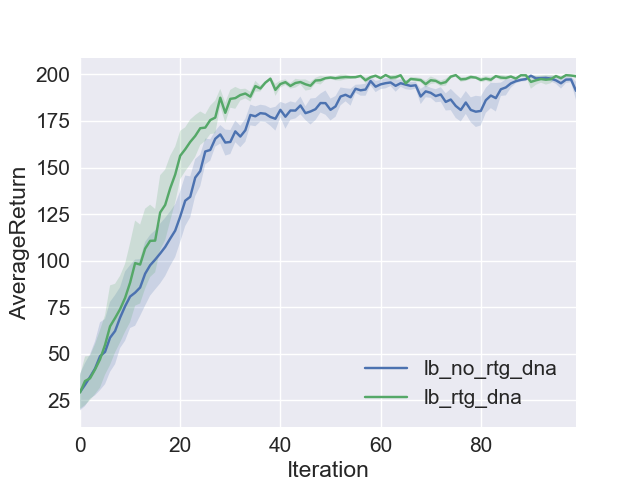
\includegraphics[width=\linewidth]{figures/lb_experiments_1.png}
  \caption{CartPole (batch size 5000)}
  \label{lb comparisons}
\end{figure}





\section*{4.2: Inverted Pendulum}

\subsection*{Methods}

For the inverted pendulum environment, I used a larger network (2 hidden layers with 64 units each) and a faster learning rate (0.01). 

\begin{knitrout}
\definecolor{shadecolor}{rgb}{0.969, 0.969, 0.969}\color{fgcolor}\begin{kframe}
\begin{alltt}
python train_pg.py InvertedPendulum-v1 -n 100 -b 4000 -rtg \textbackslash{} 
--exp_name mb_no_rtg_dna --learning_rate=0.01 --seed 101 --n_layers 2 --size 64

python plot.py data/mb_no_rtg_dna_InvertedPendulum-v1_19-09-2017_22-19-57


\end{alltt}
\end{kframe}
\end{knitrout}

\subsection*{Results}

I was able to achieve maximum performance (1000) in under 100 iterations. However, after achieving maximum performance, it still has a pretty high variance in returns. Perhaps this is due to my relatively high learning rate. See figure 3. 


\begin{figure}
  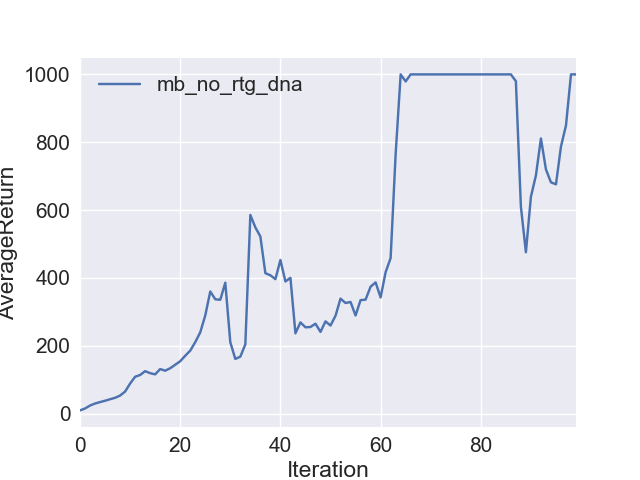
\includegraphics[width=\linewidth]{figures/inverted_pendulum_3.png}
  \caption{Inverted Pendulum}
  \label{pendulum3}
\end{figure}


\section*{5.: Inverted Pendulum with Neural Net Baselines}

\subsection*{Methods}

I used the same parameters as before for the Inverted Pendulum. I compared with and without using a neural network to predict the baseline. 

\begin{knitrout}
\definecolor{shadecolor}{rgb}{0.969, 0.969, 0.969}\color{fgcolor}\begin{kframe}
\begin{alltt}
python train_pg.py InvertedPendulum-v1 -n 100 -b 4000 -rtg \textbackslash{} 
--exp_name mb_no_rtg_dna_baseline --learning_rate=0.01 \textbackslash{} 
--seed 101 --n_layers 2 --size 64 --nn_baseline

python plot.py \textbackslash{} 
data/mb_rtg_dna_InvertedPendulum-v1_19-09-2017_22-19-57 \textbackslash{} 
data/mb_rtg_dna_baseline_InvertedPendulum-v1_19-09-2017_22-33-05


\end{alltt}
\end{kframe}
\end{knitrout}

\subsection*{Results}

With this random seed and single run, using baseline's actually improved the rate of convergence and the assymptomtic variance. If I had more time today, I would have run several experiments to see if this result holds across multiple random seeds. See figure 4.

\begin{figure}
  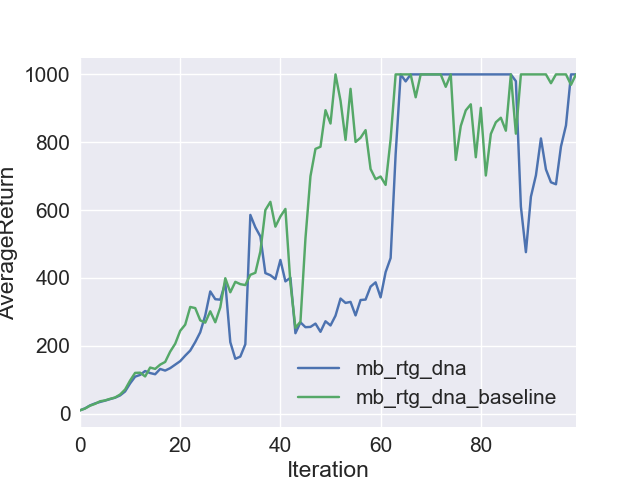
\includegraphics[width=\linewidth]{figures/inverted_pendulum_baseline_exp.png}
  \caption{Inverted Pendulum}
  \label{pendulumas}
\end{figure}

\section*{6.: Half Cheetah}

\subsection*{Methods}

I started with a small batch size and small network and then increased the size of each. Increasing batch size and the network genarally increased the average reward by iteration 100. Increasing the learning rate beyond 0.01 tended to make things unstable. I tried baseline prediction with smaller batch size, but since it did not seem to help much, I stopped using it for larger batch size (to save time). 


\begin{knitrout}
\definecolor{shadecolor}{rgb}{0.969, 0.969, 0.969}\color{fgcolor}\begin{kframe}
\begin{alltt}

python train_pg.py HalfCheetah-v1 -n 100 -b 35000 -rtg -ep 150 --discount 0.9 \textbackslash{}
--exp_name mb_no_rtg_dna --learning_rate=0.01 --seed 102 --n_layers 3 --size 128

python plot.py data/mb_no_rtg_dna_HalfCheetah-v1_20-09-2017_20-51-02


\end{alltt}
\end{kframe}
\end{knitrout}


\subsection*{Results}

My policy gradient implementation achieves 143 by iteration 100 of the algorithm (just shy of the target). A few more iterations and it would have been over. A larger batchsize and network did help. See Figure 5.


\begin{figure}
  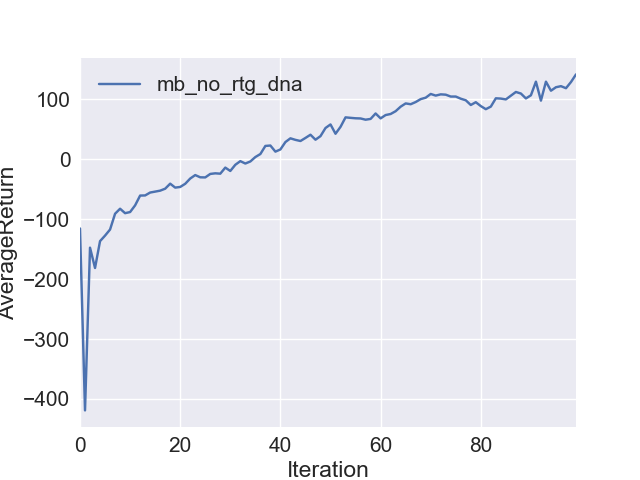
\includegraphics[width=\linewidth]{figures/cheetah_6.png}
  \caption{Half Cheetah}
  \label{cheetah}
\end{figure}



\end{document}
